% !TEX root = ../main.tex

\chapter{Temps-réel et interférences}

Dans le chapitre précédent, nous avons vu que les processeurs multi-cœurs COTS présentent le problème des interférences dues au partage de matériel entre les cœurs.
Ces interférences étant à l'origine de ralentissements pour les applications s'exécutant en parallèle, elles posent particulièrement problème dans les systèmes temps-réel.
Ce chapitre expose les problématiques liées à l'utilisation de processeurs multi-cœur COTS dans ce type de système.

Ce chapitre est organisé de la façon suivante. 
Dans la première section, on expose des généralités sur les systèmes temps-réels, notamment sur les contraintes que ceux-ci doivent respecter.
Dans la deuxième section, nous présentons les différentes approches employées pour s'assurer du respect de ces contraintes.
Dans la troisième section, nous exposons les conséquences qu'ont les interférences dans la mise en œuvre de ces méthodes d'analyses.
Enfin, dans la quatrième et dernière section de ce chapitre, nous faisons un état de l'art des approches proposées pour la gestion du problème des interférences dans les systèmes temps-réels.

%\section{Systèmes embarqués temps-réel}

% Un système temps-réel se compose d'une ou plusieurs fonctionnalités (ou sous-systèmes) devant répondre dans un temps borné à des stimuli extérieurs.
% Le principal enjeu dans la conception d'un tel système est de s'assurer que son temps de réponse est prédictible.
% Des méthodes d'analyses ont été développées de garantir la réactivité de ces systèmes.
% Le problème qui se pose aujourd'hui est que ces méthodes sont difficiles à mettre en œuvre sur des systèmes hébergés avec du matériel moderne, à plus forte raison s'il est affecté par les interférences.

% Ce chapitre présente les systèmes temps-réel, les techniques utilisées pour guarantir la réactivité de ces systèmes, l'impact qu'ont les interférences sur leur mise en oeuvre et différentes approches proposées par la communauté pour tenter de relever les nouveaux défils posés par les interférences.


%Dans cette section, nous détaillons les systèmes temps-réels et l'implication des interférences mémoires sur ces derniers.
%Nous présenterons d'abord les deux types d'architectures embarqués et les contraintes qu'elles apportent.
%Nous présenterons ensuite les contraintes temps-réels, et le processus utilisé jusqu'à présent pour garantir le respect de ces contraintes.
%Finalement, nous nous pencherons plus en détail sur l'analyse de pire temps d'exécution.

% \section{Généralités sur les systèmes embarqués temps-réel}

% \subsection{Architecture des systèmes embarqués}

% Un système embarqué assure un certain nombre de \emph{fonctionalité} s'exécutant sur des \emph{calculateurs} reliés entre eux par le biais d'un réseau.
% Une propriété importante à maintenir est la \emph{composabilité} des fonctionnalités.
% Un système est composable si le comportement temporel et fonctionel d'une fonctionalité n'est pas affecté par celui des autres fonctionnalités du système.
% Dans ce document, sauf mention contraire, nous nous focaliserons sur le comportement temporelle des fonctionalités et parlerons donc de \emph{composabilité temporelle}.

% L'architecture d'un système embarqué définit le placement des fonctionnalités sur les différents calculateurs.
% Il y en a deux:
% \begin{itemize}
% 	\item \emph{Systèmes fédérés} Chaque fonctionnalité occupe un calculateur dédié.
% 	Cette architecture est idéale pour la composabilité, vu que les fonctionnalités sont isolées physiquement.
% 	Elle est par contre coûteuse à mettre en œuvre, la rendant difficilement applicable pour des systèmes offrant un grand nombre de fonctionnalités.

% 	\item \emph{Systèmes intégrés} Plusieurs fonctionnalités peuvent occuper un même calculateur.
% 	Cette architecture a l'avantage de réduire le coût d'implantation du système en mutualisant les calculateurs.
% 	Elle pose néanmoins le problème de garantir la composabilité du système.
% \end{itemize}

% \begin{figure}[!h]
% 	\centering
% 	\begin{subfigure}{0,4\linewidth}
% 		\centering
% 		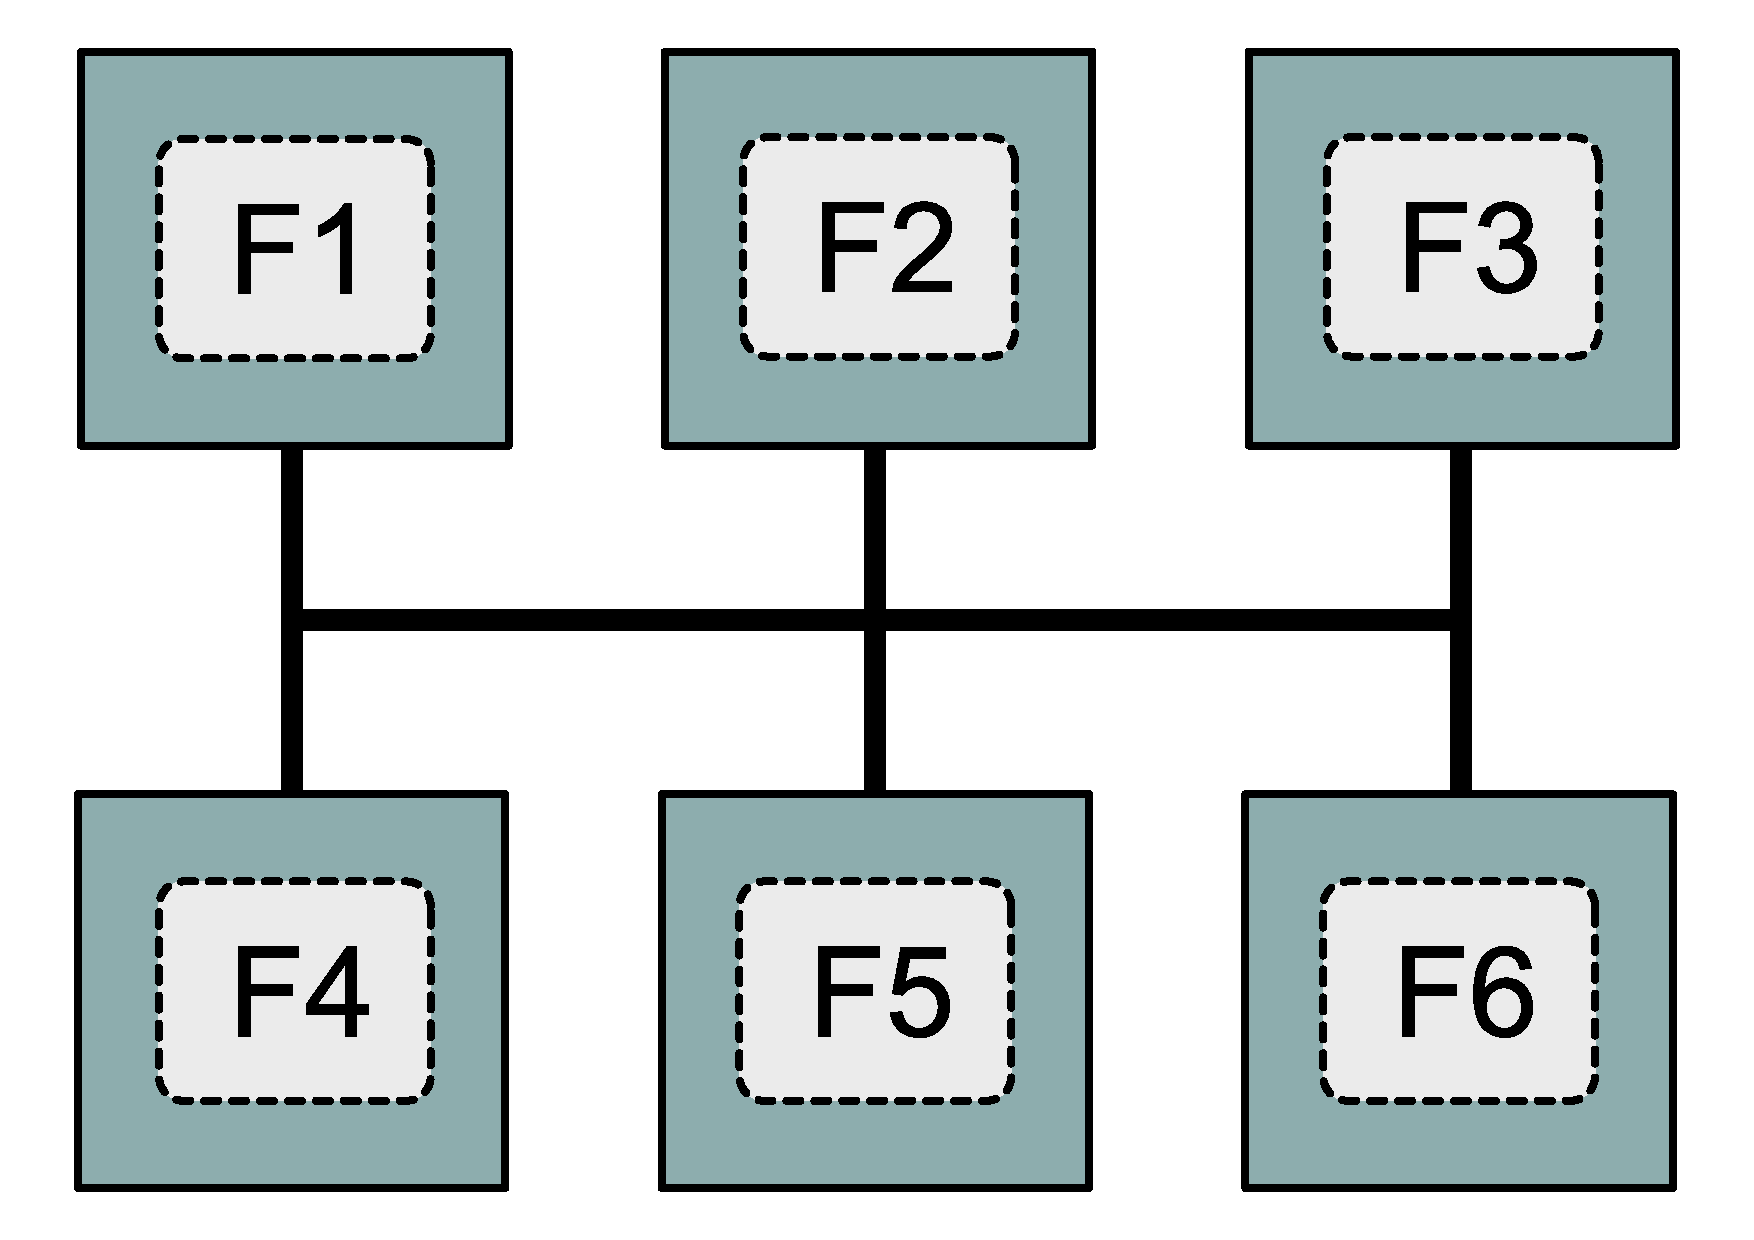
\includegraphics[width=\linewidth]{graphics/figures/federated.pdf}
% 		\caption{\label{fig:federe}Système fédéré}
% 	\end{subfigure}
% 	\begin{subfigure}{0,4\linewidth}
% 		\centering
% 		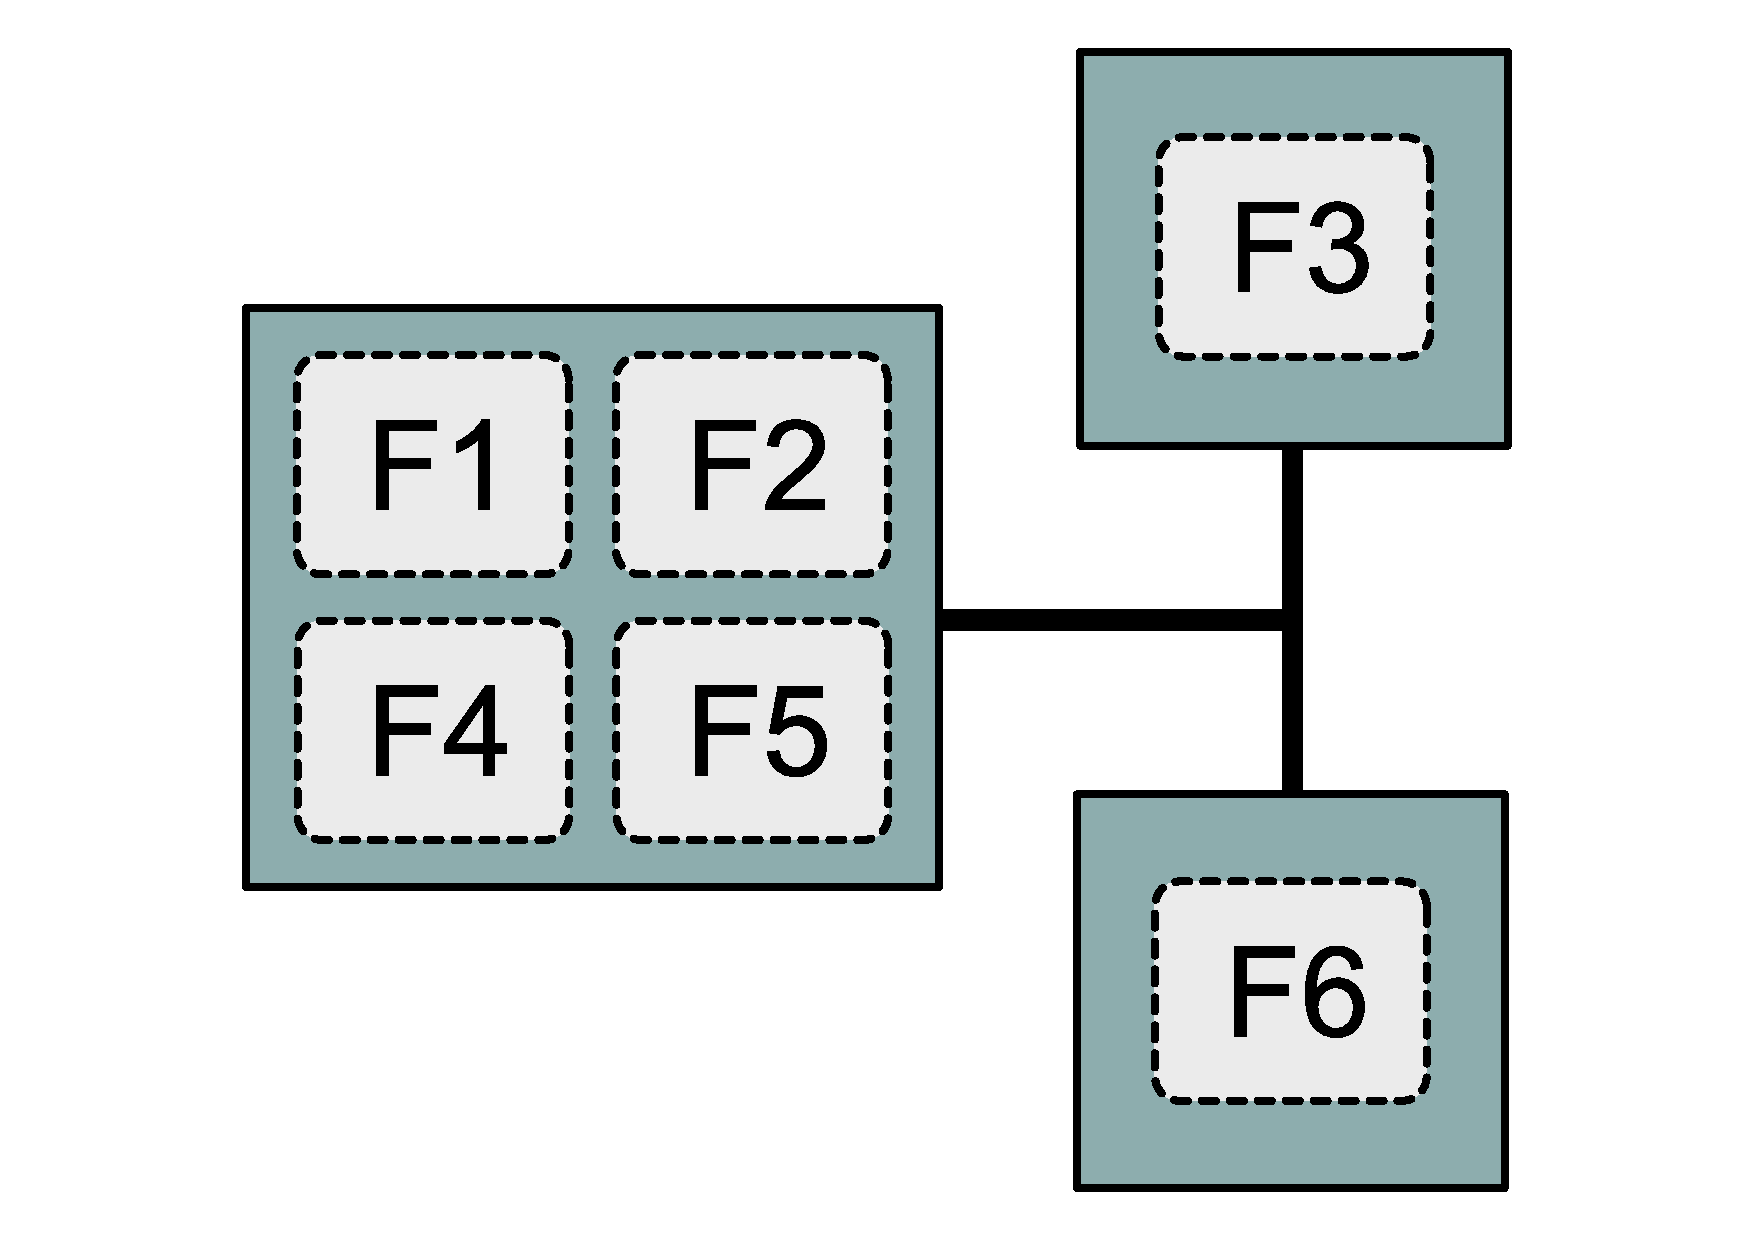
\includegraphics[width=\linewidth]{graphics/figures/integrated.pdf}
% 		\caption{\label{fig:integre}Système intégré}
% 	\end{subfigure}
% 	\caption{\label{fig:integre_federe}Architectures de systèmes embarqués}
% \end{figure}

% En théorie, l'utilisation de processeur multi-coeur offre la possibilité de pousser plus loin l'intégration des systèmes, en permettant l'exécution en parallèle de plusieurs fonctionalité sur le même calculateur.
% En pratique, malheuresement, la présence d'interférence dans les cartes multi-coeurs ne permet pas de garantir la composabilité temporelle.
% Le comportement temporel d'une fonctionalité étant alors directement affecté par les fonctionalité s'exécutant en parallèle.
% Ce problème ne permet pas d'utiliser tel quel les architectures intégrées utilisées en mono-coeur, tel qu'AUTOSAR pour l'automobile ou IMA pour l'avionique.

% Dans la section suivante, nous allons nous pencher sur l'aspect \emph{temps-réel} souvent associé aux systèmes embarqués.

% % Nous considérerons le cas, où on utilise du matériel multi-cœur pour implanter des \emph{systèmes intégrés asymétriques}.
% % À un moment donné, une fonctionnalité ne peut donc occuper qu'un seul cœur, et le but est d'exécuter plusieurs fonctionnalités en parallèle.
% % Le problème que pose la présence d'interférences est que la composabilité temporelle du système n'est plus assurée.
% % Cela a des implications pour garantir les propriétés temps-réels, nous allons maintenant voir lesquels.

\section{Généralités sur les systèmes temps-réels}

Un \emph{système temps-réel} est un système comprenant des tâches devant respecter des \emph{échéances}.
Cela ne signifie pas que le temps de réaction doit être rapide, mais qu'il doit être \emph{borné}.
Le modèle couramment utilisé, introduit par Liu et Layland~\cite{liu1973scheduling}, définit un système temps-réel comme un ensemble de \emph{tâches périodiques}.
Une tâche y est caractérisée par une période, une échéance, et une capacité qui est le temps nécessaire à l'exécution de la tâche.
Chaque tâche est activée au début de sa période et doit se terminer avant son échéance.
Si l'échéance est dépassée, cela se traduit soit par une invalidation du résultat de la tâche (on parle alors de \emph{temps-réel dur}), soit par une dégradation de la qualité de service du système (on parle de \emph{temps-réel mou}).

Un des enjeux majeurs de la conception d'un système temps-réel est d'en garantir la \emph{sûreté temporelle}, c'est-à-dire s'assurer que toutes les tâches du système respectent leurs échéances.
Le procédé usuel consiste en deux analyses successives.

\begin{enumerate}
	\item \emph{L'analyse de pire temps d'exécution} dont le but est de dimensionner les capacités des tâches du système avec le plus long temps d'exécution possible.
	\item \emph{L'analyse d'ordonnancement} dont le but est de déterminer le temps de réponse des tâches du système pour une politique d'ordonnancement donnée.
\end{enumerate}

Un système est dit \emph{ordonancable} si on peut montrer  que le temps de réponse de toutes les tâches du système est inférieur ou égal à son échéance.
Un exemple de système ordonancable et son ordonnancement est donné figure~\ref{fig:exemple_ordonancement_tr}.

\begin{figure}
	\begin{subfigure}{0,6\linewidth}
		\centering
		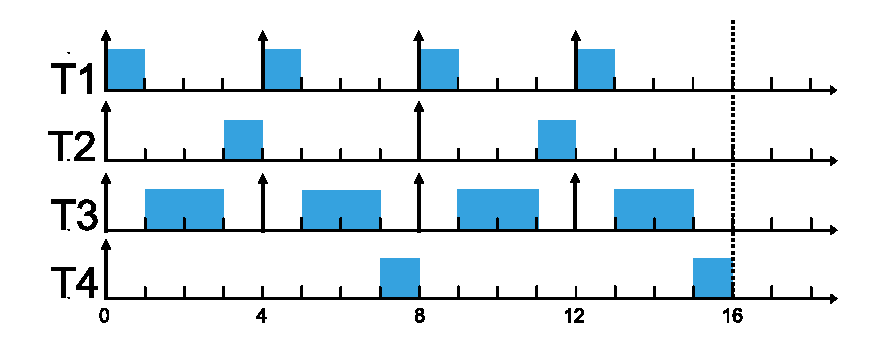
\includegraphics[width=\linewidth]{graphics/figures/sched_rt.pdf}
	\end{subfigure}
	\begin{subfigure}{0,4\linewidth}
		\centering
		\resizebox{0.9\linewidth}{!}{
			\begin{tabular}{r c c c c}
			\toprule
			& T1 & T2 & T3 & T4 \\
			\midrule
			Période  & 4 & 8 & 4 & 16 \\
			Capacité & 1 & 1 & 2 & 2  \\
			Échéance & 4 & 8 & 4 & 16 \\
			\bottomrule
			\end{tabular}
		}
	\end{subfigure}
	\caption{\label{fig:exemple_ordonancement_tr}Exemple d'ordonnancement obtenu avec la politique \emph{Earliest Deadline First}.}
\end{figure}

Ce processus repose sur une hypothèse forte, qui est que le pire temps d'exécution d'une tâche est indépendant des autres tâches du système.
En d'autres termes, il repose sur la composabilité du système. Or, nous avons vu que cette dernière n'est pas assurée en présence d'interférences.
Le choix du matériel a donc un impact important sur l'analyse de pire temps d'exécution.
C'est ce problème que nous allons étudier dans le reste de ce chapitre.

\section{Analyse de pire temps d'exécution en mono-cœur}

Dans un système temps-réel, on suppose que la capacité des tâches correspond au temps nécessaire au parcours de leur plus long chemin d'exécution\footnote{La longueur est ici exprimée en temps} sur une plateforme matérielle donnée.
Ce temps est désigné par le terme \emph{WCET}\footnote{Worst Case Execution Time}(figure~\ref{fig:terminologie_wcet}).
Le but de l'analyse de pire temps d'exécution est de borner le WCET.
Cette analyse se doit d'être \emph{sûre} et \emph{précise} : le WCET estimé ne doit pas être inférieur au WCET réel (sûreté) et il doit s'en approcher autant que possible (précision).

% L'analyse de pire temps d'exécution a pour but de déterminer le pire temps d'exécution (\emph{Worst Case Execution Time ou WCET}) d'une tâche sur un matériel donné.
% Comme illustré dans la figure~\ref{fig:terminologie_wcet}, cela que l'on cherche à déterminer le temps d'exécution le plus long parmi tous les temps d'exécution possibles.
% Le but de l'analyse est de calculer une borne sur le WCET qui soit à la fois sûre et précise.
% La sûreté se traduit par le fait que la borne ne doit pas être inférieure au WCET réel de la tâche, il s'agit d'un critère de correction de l'analyse.
% La précision est atteinte si la borne calculée est proche du WCET réel, il s'agit alors d'un critère de performance de l'analyse. 

\begin{figure}[!h]
	\centering
	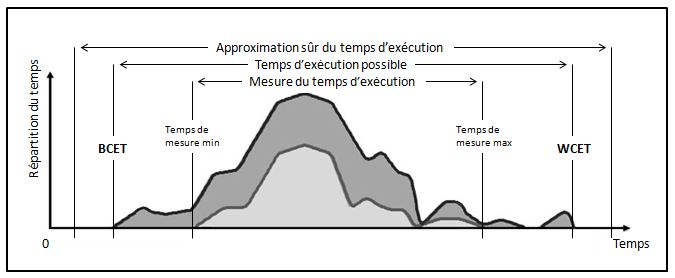
\includegraphics[width=\linewidth]{graphics/figures/termes_wcet.jpg}
	\caption{\label{fig:terminologie_wcet}
	Résumé des notions concernant l'analyse de pire temps d'exécution.
	La courbe la plus haute représente l'ensemble de toutes les exécutions possibles, tandis que la courbe la plus basse représente un sous-ensemble d'exécution mesurée.
	 (Source de l'illustration : Wikipedia)}
\end{figure}

% Il y a deux grandes familles d'approches, que nous allons maintenant détailler, pour l'analyse de pire temps d'exécution: celles basées l'analyse statique et les approches dynamiques.

Nous allons maintenant détailler deux grandes familles d'analyse du pire temps d'exécution : celles basées sur l'analyse statique de l'application (on parle de méthodes statiques) et celles basées sur des mesures (on parle de méthodes dynamiques).

\subsection{Méthodes statiques}

Les analyseurs statiques~\cite{ferdinand2004ait,lisper2014sweet,rapitime,ballabriga2010otawa,li2007chronos} de WCET le calculent sans exécuter directement les tâches. 
Une architecture générale de l'analyse employée par ces outils est décrite par Wilhelm et al.~\cite{wilhelm2009memory} et résumée par la figure~\ref{fig:process_wcet}.

\begin{figure}[!h]
	\centering
	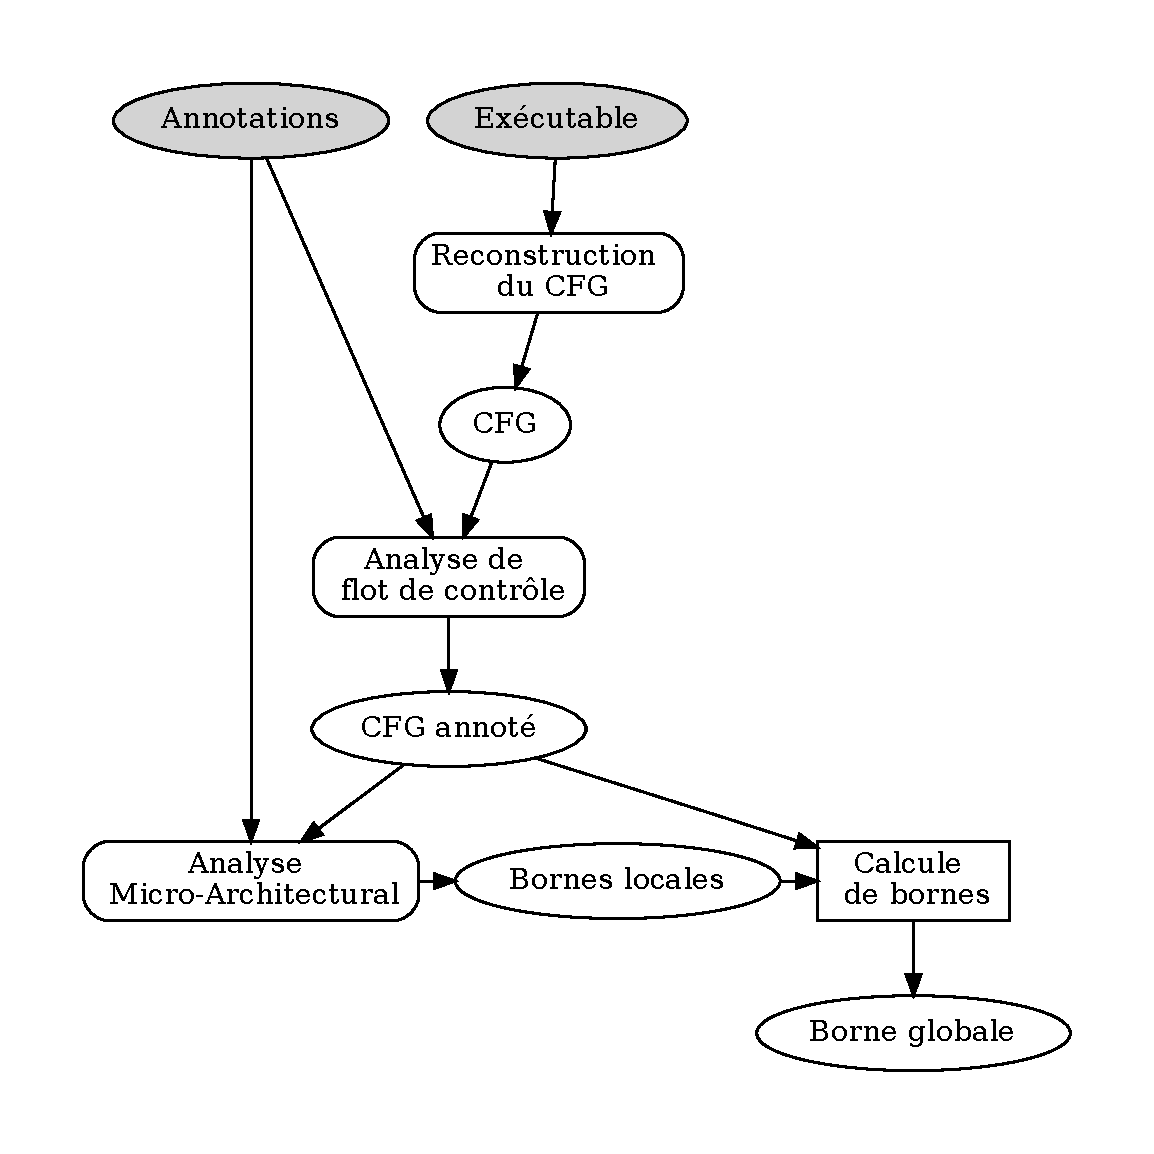
\includegraphics[width=\linewidth]{graphics/figures/wcet_static.pdf}
	\caption{\label{fig:process_wcet}Analyse statique de pire temps d'exécution}
\end{figure}

Les points d'entrée de ce type d'analyse sont le fichier binaire exécutable de la tâche analysée et un ensemble d'informations complémentaires sous forme d'annotations.
Ces informations peuvent décrire l'agencement de la mémoire, l'intervalle de valeur d'entrées de la tâche, des informations sur son flot de contrôle, etc.
Le processus de calcul de WCET à partir de ces éléments est le suivant :

\begin{enumerate}
	\item \emph{Reconstruction du graphe de flots de contrôle} Le flot de contrôle est reconstruit à partir du binaire afin d'extraire une représentation intermédiaire pour la suite de l'analyse.
	Cette étape est comparable à un frontend de compilateur.
	Le produit de cette étape est donc un \emph{graphe de flot de contrôle (CFG)}.
	
	\item \emph{Analyse du flot de contrôle} Le CFG est analysé afin de construire l'ensemble des chemins d'exécutions pouvant être possiblement être emprunté par la tâche.
	Un des objectifs de cette étape est d'éliminer de façon sûre le plus de chemins possible.
	Le produit de cette étape est un CFG annoté avec des contraintes sur le comportement dynamique de la tâche.

	\item \emph{Analyse micro architecturale} Une borne sur le temps d'exécution des blocs de bases du CFG sont calculés en utilisant un modèle abstrait du matériel.
	Le produit de cette étape est un ensemble de \emph{bornes locales}.

	\item \emph{Calcul de la borne global} Finalement, les bornes locales et les informations sur le flot de contrôle sont utilisées pour déterminer la \emph{borne globale} sur le pire temps d'exécution de la tâche.
\end{enumerate}

\subsection{Méthodes dynamiques}

L'analyse dynamique de pire temps d'exécution utilise des expériences pour déterminer le pire temps d'exécution d'une tâche.
Elle peut s'effectuer aussi bien de bout en bout que par morceau.
Dans l'analyse de bout en bout, c'est le temps complet d'une exécution de la tâche qui est mesuré.
Tandis que dans l'analyse par morceau, les mesures sont effectuées sur les blocs de bases de l'application.

Qu'elles soient de bout en bout ou par morceaux, l'analyse dynamique de pire temps d'exécution est généralement considérée comme non sûre.
D'une part, il faut s'assurer que le chemin correspondant au WCET est bien couvert par les mesures, ce qui n'est en général pas possible avec les processeurs modernes.
Ainsi, si l'on se réfère à la terminologie de la figure~\ref{fig:terminologie_wcet}, l'analyse de bout en bout ne permet techniquement d'obtenir \emph{qu'un pire temps d'exécution observé}.
Elles peuvent néanmoins être utilisées pour étudier la variabilité des temps d'exécution d'une tâche, ou encore pour valider les résultats de l'analyse statique.

\subsection{Défis de l'analyse de pire temps d'exécution}

Qu'elle soit statique ou dynamique, la complexité de mise en œuvre de l'analyse de pire temps d'exécution est fortement liée à la complexité du matériel.

Le chemin d'exécution avec le WCET dépend à la fois des données en entrée de la tâche et de l'état dans lequel se trouve le matériel.
Ces deux données étant en général difficiles à déterminer à l'avance.
Plus le matériel est complexe, plus le nombre d'états dans lequel celui peut se trouver (et donc le nombre de cas à considérer) est grand.
Cela entraine des problèmes d'explosion combinatoire concernant aussi bien les méthodes statiques (il faut considérer plus de cas dans l'analyse) que les méthodes dynamiques (la couverture de tests à fournir est plus grande).
% Cela se traduit par un problème d'explosion combinatoire dans les approches statiques, et par une couverture de tests difficile à atteindre dans les .

De plus, les processeurs modernes posent le problème du temps d'exécution des instructions.
En effet, ce dernier n'y est pas fixe.
Il dépend de l'historique des instructions exécutées précédemment.
D'une part, cela rend difficilement applicable l'analyse dynamique par morceau sur ce type de matériel.
D'autre part, cela complique l'analyse micro architecturale dans les approches statiques.
En effet, le modèle abstrait du matériel doit alors prendre en compte l'effet de composants tel que les pipelines ou les caches pour déterminer les bornes locales de la tâche.
Cela requiert un niveau d'information élevé sur le matériel qui n'est pas toujours disponible, à plus forte raison sur du matériel grand public.
De plus, le comportement dans le pire cas des composants peut conduire à des bornes très grandes.

Enfin, le dernier problème qui se pose est la présence d'anomalies temporelles sur le matériel récent.
Une anomalie temporelle survient lorsque le pire temps global n'est pas composés uniquement de pires temps locaux.
La figure~\ref{fig:anomalie} illustre un exemple d'anomalie causé par le réordonnancement des instructions au sein du pipeline d'un processeur.
On peut y voir deux ordonnancements d'instructions partiellement dépendantes entre elles.
Les séquences sont identiques à l'exception de l'instruction A qui met plus de temps à s'exécuter dans le premier cas que dans le second.
L'anomalie est que c'est ce dernier cas qui met le plus de temps à s'exécuter au final.
Si on ne peut pas borner \emph{par une constante} la différence de temps d'exécution causée par les anomalies temporelles, on parle alors d'\emph{effet domino}.
Les processeurs modernes présentent en général à la fois des anomalies temporelles et des effets dominos.
La présence d'anomalie temporelle a plusieurs conséquences:
\begin{itemize}
	\item Il n'est pas sûr d'utiliser l'approche gloutonne pour déterminer le chemin d'exécution correspondant au WCET.
	\item On ne peut pas identifier un pire état initial, permettant par exemple de procéder de façon sûre à de l'analyse dynamique par morceau.
	\item Une architecture matérielle présentant des anomalies temporelles et des effets dominos est dite \emph{non-compositionelle}~\cite{hahn2015towards}.
	Une architecture est compositionnelle si on peut décomposer le pire temps d'exécution totale en la somme des contributions au pire temps d'exécution des éléments du système.
	La conséquence est que l'on ne peut pas modulariser aisément l'analyse de ce genre de matériel.
\end{itemize}

\begin{figure}
\centering
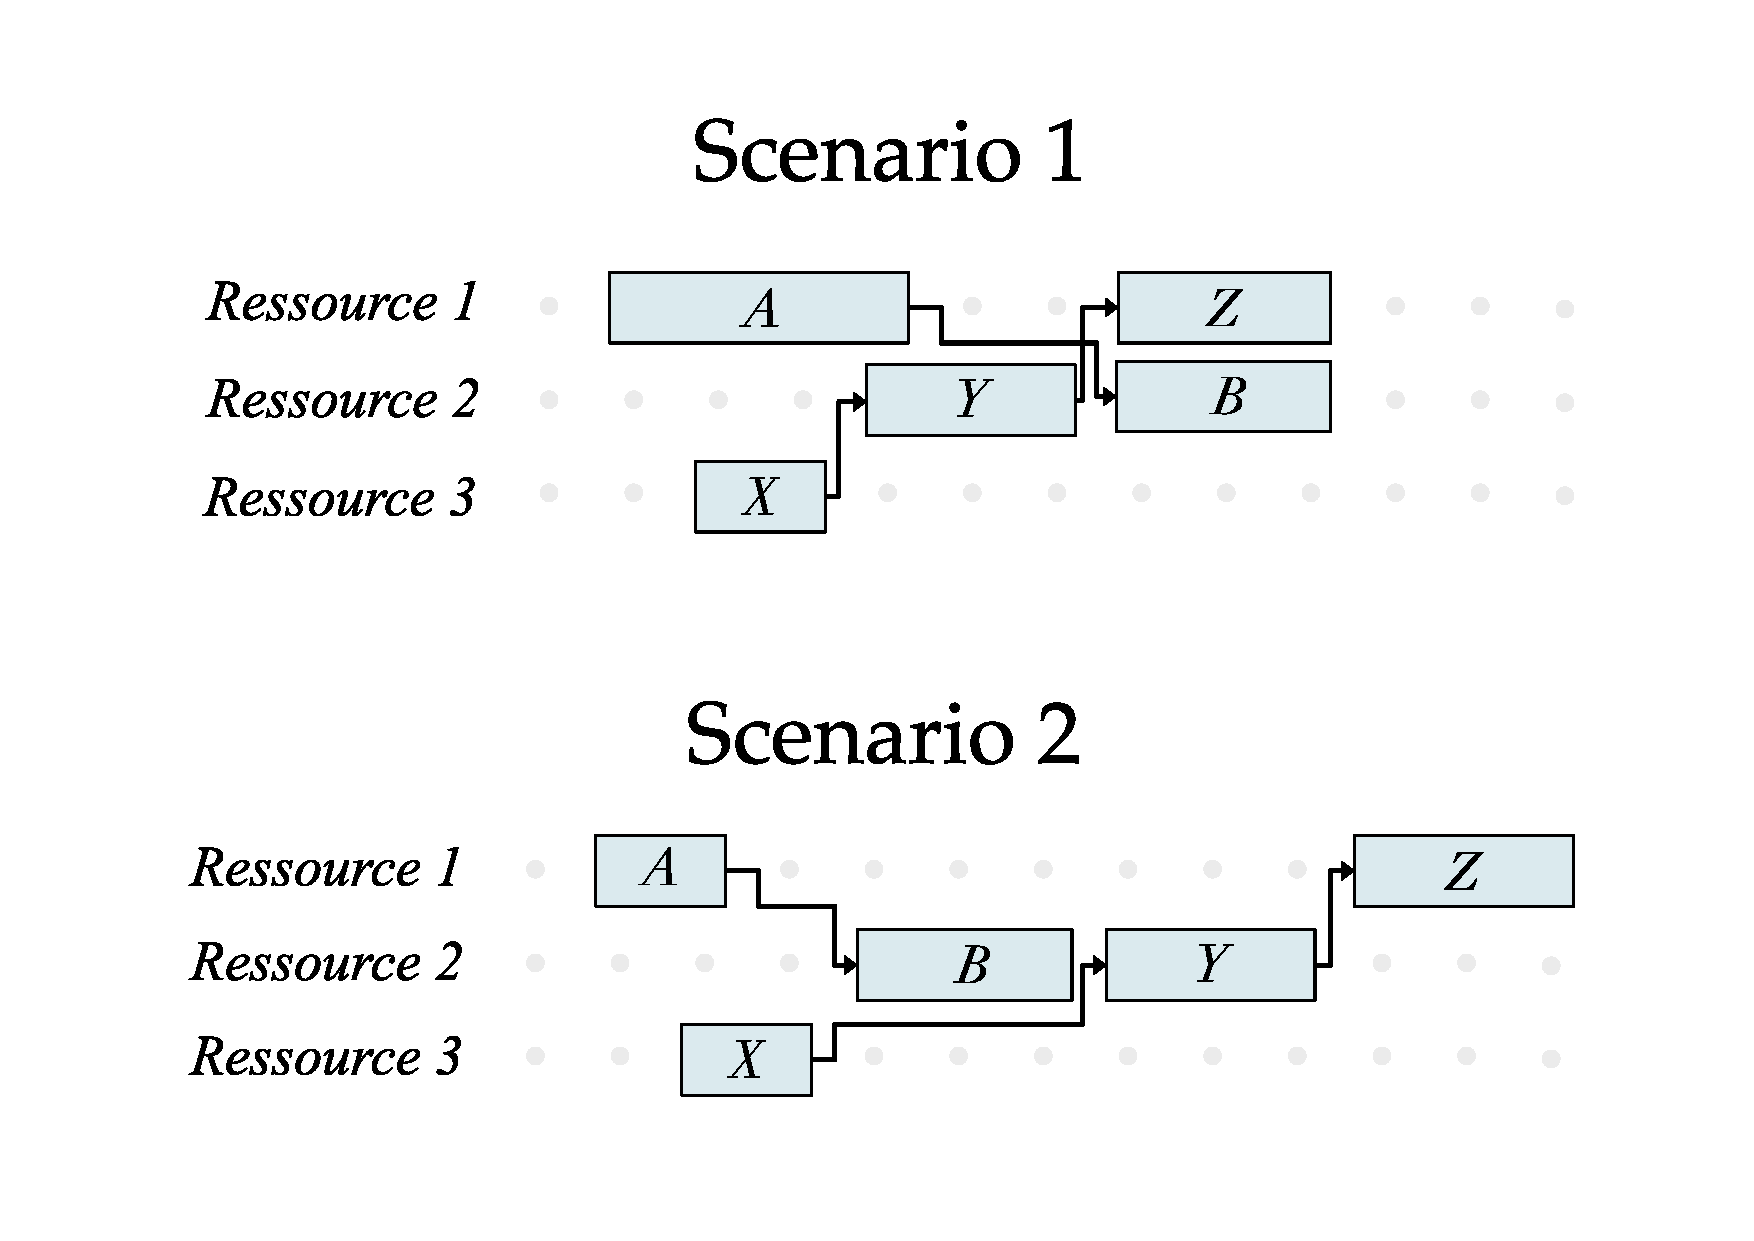
\includegraphics[width=0.7\linewidth]{graphics/figures/anomalie2.pdf}
\caption{\label{fig:anomalie} Exemple d'anomalie temporelle due à un réordonnancement d'instructions. Les flèches indiquent des dépendances entre instructions.}
\end{figure}

\section{\label{section:impact-interferences-wcet}Impact des interférences}

L'utilisation de matériel multi-cœur COTS a un impact très important dans le cadre des systèmes temps-réels.
Elle remet notamment en question l'applicabilité des méthodes existantes pour vérifier la sûreté temporelle de ces systèmes.

Les interférences peuvent causer des ralentissements plus ou moins importants aux tâches temps-réels, qui s’ ils ne sont pas pris en compte peuvent causer un sous-dimensionnement du système entrainant des dépassements d'échéances.
Le ralentissement subi par une tâche dépend à la fois de son utilisation du système mémoire, mais aussi de la pression exercée sur celui-ci par les autres tâches du système.
Dans ces conditions, il devient  difficile d'évaluer le pire temps d'exécution indépendamment du contexte d'ordonnancement, remettant ainsi en cause l'approche en deux étapes utilisées dans les systèmes mono-cœurs.
Notons également que dans des systèmes à criticité mixte, le comportement exact des tâches non critique n'est en général pas connu, empêchant ainsi l'évaluation du contexte d'ordonnancement.

La nature du matériel utilisé pose également problème.
Tout d'abord, les processeurs multi-cœurs COTS sont en général très complexes et leur comportement n'est en général pas documenté exhaustivement.
Dans ces conditions, construire un modèle abstrait d'un tel processeur est difficile et peut conduire à l'utilisation d'hypothèses simplificatrices souvent très pessimistes.
Ensuite, ces processeurs sont conçus pour offrir de bonnes performances en moyenne, et donc le comportement des mécanismes utilisés peut être très mauvais dans les pires cas.
Enfin, la non-compositionnalité des architectures employées aggrave encore ce problème, dans la mesure où elle complique la modularisation de l'analyse.

Dans les faits, les points que nous venons de soulever entrainent l'adoption d'hypothèse très pessimistes, et donc le surdimensionnement des systèmes.
D'un point de vue industriel, tout l'enjeu est de pouvoir dimensionner de façon sure, mais aussi efficace, les systèmes temps-réel en tenant compte des interférences.
Dans la section suivante, nous allons présenter l'état de l'art des interférences.

\section{Temps-réel et interférences}

% Les méthodes utilisées jusqu'alors pour s'assurer du respect des contraintes temporelles ont initialement été dévelopée pour des systèmes mono-coeurs.
% En particulier, le pire temps d'exécution des tâches est déterminé en \emph{isolation}. 
% C'est à dire que ce temps ne varie pas en fonction du contexte d'ordonancement.
% Cette hypothèse est évidement invalidée dans le cas de système multi-coeur utilisant du matériel sujet aux interférences.
% Ne pas prendre l'effet de ces interférences peut conduire à sous-estimer le pire des tâches temps-réels, et donc conduire à des dépassement d'échéances.

% Les interférences posent un sérieux problème d'allocation de ressources dans les systèmes temps-réels.
% À cet effet, elles font partie des préocupations de la communauté temps-réels depuis la fin des années 2000.
% L'enjeu est de pouvoir dimensionner les systèmes temps-réels de façon sure et efficace.
% C'est à dire que le surcoût temporel estimé ne doit pas excéder les bénéfices apportés par le matériel.
% Dans cette section, nous allons présenter l'état de l'art de la gestion des interférences pour le temps-réel.
% Nous traiterons d'abords des travaux visant à calculer le surcout induit par les interférences.
% Nous nous pencherons ensuite sur les approches visant à isoler les applications s'exécutant en parallèle.
% Finalement, nous présenterons des solutions de régulation visant à fournir un filet de sécurité.

La présence d'interférences dans le matériel moderne fait partie des préoccupations de la communauté temps-réel depuis la fin des années 2000.
Nous allons, dans cette section, présenter diverses approches proposées pour apporter des solutions à ce problème.
Nous distinguerons trois grandes familles d'approches:
\begin{itemize}
	\item Les approches traitant du \emph{dimensionnement} du système en prenant en compte l'impact des interférences. Cela passe par l'extension des méthodes classiques de vérification temporelles, mais également par des études empiriques.

	\item Les approches traitant de \emph{l'isolation} des applications ont pour but de réduire, voir supprimer, les interférences. Elles peuvent aussi permettre un dimensionnement moins pessimiste des systèmes. 

	\item Les approches traitant de \emph{la régulation} ont pour but de fournir un filet de sécurité à l'exécution. Ces approches reposent sur un monitorage de l'état du système afin de détecter des situations pouvant causer des défaillances, et le cas échéant prendre des mesures appropriées.
\end{itemize}

\subsection{Calcul de pire temps d'exécution}

Un grand nombre de travaux visent à incorporer l'impact des interférences dans les analyses temporelles classiques.
L'enjeu de ces travaux est d'offrir des analyses à la fois sûres et efficaces : sûre, car l'impact des interférences ne doit pas y être sous-estimé, efficace, car il doit être aussi proche que possible de la réalité.
% c'est à dire que l'impact ne doit pas être sous estimé mais également aussi proche que possible de la réalité.
Il s'agit d'un problème difficile pour les raisons invoquées dans la section~\ref{section:impact-interferences-wcet}.
Le problème est d'ailleurs encore ouvert.
Pour un inventaire récent et détaillé des recherches dans ce domaine, nous orientons le lecteur vers l'étude de Maiza et al.~\cite{maiza2018survey} en complément de ce chapitre.

Les travaux étendant la vérification des propriétés temporelles des systèmes temps-réels se distinguent à la fois par le choix de l'analyse étendue (de pire temps d'exécution ou d'ordonnancement) et la modélisation des interférences.

% La transpositions des méthodes de vérifications temporelles utilisées dans les systèmes mono-coeurs aux systèmes multi-coeurs est un problème difficile, faisant d'ailleurs encore aujourdh'ui l'objet d'un effort important de recherche.
% Une étude détaillée sur les dernières avancées dans ce domaine a été proposée par Maiza et al.~\cite{maiza2018survey}.
% Les travaux se distinguent aussi bien par le type d'analyse étendue(de pire temps d'exécution que de l'analyse d'ordonancement) que par la modélisation des interférences.

\paragraph{Extension de l'analyse de pire temps d'exécution}
Peu de travaux incorporent les interférences dans l'analyse de pire temps d'exécution. 
Cela peut s'expliquer par l'absence de contexte d'exécution, rendant difficile la modélisation des interférences.
On peut néanmoins, prendre en compte les interférences dans cette analyse en suivant deux approches:
\begin{itemize}
	\item L'\emph{approche de Murphy}~\cite{abel2013impact}\footnote{Nommée d'après la loi éponyme.} consiste à considérer toutes les interférences possibles pour chaque accès.
	Pour pouvoir appliquer cette approche, le pire surcoût possible par accès doit être borné.
	Ce n'est pas toujours possible, et dans le cas où on pourrait le faire, les bornes calculées sont en général très pessimistes~\cite{perret2016predictable,nowotsch2014multi}.

	\item Les \emph{approches complètement intégrées} visent à analyser simultanément toutes les tâches s'exécutant en parallèle.
	Ce type d'analyse offre théoriquement une précision idéale, le surcoût temporel estimé étant déterminé à partir de tous les entrelacements d'accès possible sur les ressources partagées.
	En pratique, l'applicabilité de ce type d'approche reste incertaine.
	En cause le niveau d'information requis sur toutes les tâches du système, mais aussi la complexité du calcul.
\end{itemize}

\paragraph{Extension de l'analyse d'ordonnancement}
Les interférences peuvent également être intégrées dans le calcul du pire temps de réponse.
C'est-à-dire pendant l'analyse d'ordonnancement.
Cette approche permet de prendre en compte le contexte d'ordonnancement, en particulier la pression éventuelle sur les ressources partagées.
Néanmoins, lorsque ce contexte n'est pas disponible, par exemple dans le cas où le comportement des autres tâches n'est pas connu, des hypothèses pessimistes de consommation peuvent être employées.
Un certain nombre de travaux repose sur l'utilisation de \emph{courbes d'arrivée} comme abstraction de la consommation de ressources partagées.
Ces courbes sont des fonctions associant à chaque intervalle de temps le nombre d'occurrences d'un événement.
Elles permettent donc de borner quantitativement la consommation de ressource mémoire d'une tâche.
Des travaux récents~\cite{oehlert2018compiler} montrent que ces courbes peuvent être déterminées par des méthodes d'analyse statiques.

\paragraph{Modèles d'interférences des composants du système mémoire}
L'estimation de l'impact des interférences, quel que soit la méthode employée, repose sur un modèle plus ou moins détaillé du système mémoire.
Les composants étudiés dans la littérature sont les bus d'interconnexions, les caches, et la DRAM.

La principale difficulté concernant les bus d'interconnexion est le manque d'information sur la politique d'arbitrage utilisée en cas d'accès concurrents.
Notons que certaines politiques d'arbitrage n'ont pas de temps de réponse borné.
Les articles traitant des bus font en général des hypothèses sur cette politique, en considérant par exemple une politique TDMA.
Cela pose problème pour appliquer ces résultats lorsque l'on cible du matériel COTS.

Les caches ont également fait l'objet d'une attention particulière.
La majorité des travaux sont consacrés aux interférences spatiales, et donc à déterminer le nombre de défauts de caches supplémentaires induit par les interférences.
Ces approches ont d'abord été limitées aux caches d'instructions~\cite{2008_Yan_WCET_analysis_for_Multi_Core_processors_with_shared_L2_instruction_caches,zhang2009accurately,2009_hardy_using_bypass_to_tighten_WCET_estimates_for_Multi_Core_processors_with_shared_instruction_caches}, puis étendues aux caches de données~\cite{2010_Lesage_shared_data_caches_conflicts_reduction_for_WCET_computation_in_Multi_Core_architectures}.
Si dans les caches partagés, les interférences spatiales les plus évidentes, il ne faut pas oublier que les interférences temporelles existent.
Valsan et al.~\cite{valsan2016taming} ont montrés ce problème sur diverses architectures.
Mesurer précisément l'impact de ces interférences temporelles semble néanmoins difficile.

De multiples conceptions de contrôleur DRAM déterministe ont été proposées~\cite{2007_Akesson_Predator_A_predictable_SDRAM_memory_controller,2011_Reineke_PRET_DRAM_controller_bank_privatization_for_predictability_and_temporal_isolation,2014_Krishnapillai_ROC_A_rank_switching_open_row_DRAM_controller_for_time_predictable_systems}, mais peu d'études ont été effectuées sur les contrôleurs utilisés dans les plateformes COTS.
Wu et al.~\cite{wu2013worst} ont réalisé une des premières études de pire temps de réponse de la DRAM.
Les auteurs y font néanmoins l'hypothèse de l'absence de politique de réordonnancement, ces dernières pouvant conduire à des temps d'accès non bornés.
Cette hypothèse a ensuite été levée par Kim et al.~\cite{kim2014bounding,kim2016bounding}.
Les résultats de ces analyses restent pessimistes, et peuvent être surtout invalidés en fonction des politiques d'arbitrage effectivement implantées dans les contrôleurs.

La présence d'anomalies temporelles et d'effets dominos dans les architectures modernes pose également le problème de la compositionnalité des analyses d'interférences.
En effet, rien ne dit que la somme des retards dus aux interférences de chaque composant est supérieure ou égale au retard finalement observé.
Des approches pour prendre ce phénomène en compte ont été proposées par Hahn et al.~\cite{hahn2016enabling}, augmentant encore le pessimisme des analyses.
Réciproquement, la capacité de recouvrement des retards offerts par les processeurs modernes par le biais de mécanismes comme les pipelines et l'exécution dans le désordre ne sont pas pris en compte.

\subsubsection{Conclusions}

Les approches présentées dans cette section visent à borner de façon sûre l'effet des interférences.
Elles se heurtent néanmoins à la complexité et à l'opacité du matériel étudié.
Ainsi, des hypothèses simplificatrices sont souvent employées, remettant en cause l'applicabilité de ces travaux pour des cibles COTS.
Enfin, les bornes dérivées sont très pessimistes, au point de les rendre inutiles en pratique, le surcoût calculé compensant complètement le bénéfice apporté par le fait d'avoir plusieurs cœurs.

\subsection{Approches empiriques}

L'analyse statique du pire temps d'exécution est un problème difficile, dont la complexité de mise en œuvre croît avec celle du matériel ciblé.
Les processeurs évoluant plus vite que les approches d'analyse statiques, ces dernières sont aujourd'hui difficilement applicables au matériel moderne.
Cette situation explique un regain d'intérêt pour les approches empiriques, certes non sûres, mais considérablement plus aisées à mettre en œuvre.

% La difficulté de mise en oeuvre des approches statiques pour déterminer le surcoût apporté par les interférences augmente l'intéret pour les méthodes dynamiques.
% Ces dernières, certes jugées non sûre, offre l'avantage d'être considérablement plus simple à mettre en oeuvre.

Les approches empiriques ont notamment été utilisées dans un certain nombre d'études afin d'étudier l'ampleur des ralentissements que peuvent causer les interférences sur du matériel COTS.~\cite{zhuravlev2010addressing,bin2014studying,radojkovic2012evaluation,fernandez2012assessing,6214768}.
Ces études utilisent des microbenchmarks spécifiquement conçus pour stresser les composants partagés du système mémoire, on parle de \emph{charges}.
En comparant des temps d'exécution en isolation et face à des charges, on peut évaluer les retards observés en pratique sur du matériel complexe.
Ce type d'analyse n'est en principe pas sûr, vu que l'on ne peut savoir si le pire cas a effectivement été couvert.
En pratique, le comportement des charges est pessimiste, et s'apparente à une tentative de déni de service sur la mémoire.
Il est néanmoins souhaitable d'avoir des charges générant le plus d'interférences possible.
Or, les charges générant le plus de perturbations varient d'une cible matérielle à l'autre, nécessitant un effort de conception au cas par cas.
Afin de réduire cet effort, une approche automatique a été proposée par Iorga et al.~\cite{iorga2018your} pour concevoir de telles charges.

% Ainsi, il peut être désirable d'avoir des charges les plus aggressives possibles, mais celle-ci peuvent varier en fonction du matériel.
% À cet effet, une approche automatique pour déterminer les charges les plus aggressive a été proposée par Iorga et al.~\cite{iorga2018your}.

% Les méthodes empiriques d'analyse d'interférences repose sur l'utilisation de microbenchmarks destinés à mettre sous pression les différents composants partagés du système mémoire.
% Cette approche a été utilisée notamment pour estimer l'ampleur du problème des interférences~\cite{zhuravlev2010addressing,bin2014studying,radojkovic2012evaluation,fernandez2012assessing,6214768}.
% Certains de ces travaux se penchent également sur le problème de caractériser la consommation des applications.
% Bin et al.~\cite{bin2014studying} détermine notamment une signature des applications en utilisant des compteurs matériels, afin de déterminer quelles ressources sont affectées par les interférences.
% Ces approches ne permettent pas de définir une borne sur le temps d'exécution, mais d'estimer le retards subi en pratique.
% Bien que les microbenchmarks employés ont un comportement invraisemblablement aggressif, il n'y a pas de garanties qu'ils fournissent le plus grand niveau de stress possible.
% A cet effet, Iorga et al.~\cite{iorga2018your} proposent une méthode permettant de trouver des paramètre de stress optimaux.

Un autre usage des méthodes empiriques est de caractériser la sensibilité d'une application aux problèmes des interférences, principalement à des fins de dimensionnement.
On observe deux types de caractérisation:
\begin{itemize}
	\item \emph{Les approches a posteriori} caractérisent la sensibilité des applications en les soumettant à de l'injection de charges. 
	\item \emph{Les approches a priori} caractérisent la sensibilité des applications en fonction de leur comportement en isolation.
\end{itemize}

Dans les approches a posteriori, le comportement des applications est caractérisé à l'aide de l'injection de charges.
Ainsi, la sensibilité d'une application aux interférences est décrite par une courbe décrivant l'évolution du retard subi en fonction de la charge observée dans le système.
Ce type d'approche a notamment été utilisée pour la colocalisation d'applications dans les centres de données~\cite{mars2011bubble,black2013bandwidth,215971,zhao2016predicting,zhao2015predicting}.
Le but étant de constituer des groupes d'applications en minimisant les interférences.


Les approches a priori visent à inférer le retard que peut subir une application en fonction de son comportement en isolation.
Griffin et al.~\cite{griffin2017forecast} utilisent des réseaux de neurones profonds~\cite{lecun2015deep} pour cette inférence.
Le comportement en isolation est caractérisé en effectuant une analyse de composantes principales~\cite{wold1987principal} sur des données collectées à l'aide de compteurs de performances.
Cette approche a deux inconvénients.
Tout d'abord, la caractérisation reposant sur tout les événements mesurés, un grand nombre d'expériences est nécessaire.
Ensuite, en fonction des événements observable sur la machine, l'efficacité de la caractérisation peut varier fortement.

\subsubsection{Conclusions}

Les approches empiriques ont l'avantage d'être immédiatement applicables.
Elles reposent majoritairement sur de l'injection de charges pour déterminer les retards subis en pratique par des applications.
Ces méthodes sont théoriquement non sûres.
Il est en effet très difficile, sinon impossible, de s'assurer que le stress apporté par les charges correspond effectivement au pire scénario d'interférences.

\subsection{Isolation du matériel}

Nous venons d'évoquer différentes analyses de l'impact des interférences.
Une autre manière d'aborder le problème est d'empêcher les interférences en améliorant l'isolation entre les différents cœurs.
Loin de concurrencer les analyses susmentionnées, l'isolation peut offrir des hypothèses plus favorables à l'estimation de l'impact des interférences.
Nous reprenons la distinction utilisée pour catégoriser les interférences, en distinguant l'\emph{isolation spatiale} de l'\emph{isolation temporelle}.

\subsubsection{Isolation spatiale}

L'isolation spatiale est utilisée pour partitionner les différentes mémoires entre les cœurs.
On peut mettre en œuvre cette isolation par des moyens logiciels grâce à la coloration de pages, mais aussi à l'aide de support matériel, notamment dans les caches~\cite{lockdown}.

\paragraph{Coloration de pages}

La coloration de page~\cite{taylor1990tlb} désigne les politiques d'allocation de pages physiques reposant sur la notion de \emph{couleur}.
Un allocateur de page utilisant la coloration de page, associe à une adresse de page virtuelle une adresse de page physique dotée d'une couleur encodée à l'aide de certains bits d'adresse physique.
Cette technique a été utilisée en mono-cœur pour optimiser le placement de données dans les caches indexés physiquement~\cite{kessler1992page,romer1994dynamic,sherwood1999reducing,1996_bugnion_Compiler_directed_page_coloring_for_multiprocessors}.
En définissant la couleur d'une page à l'aide des bits à la fois utilisés pour définir l'adresse de page et ceux utilisés pour l'indexation dans le cache (Figure~\ref{fig:coloring}), il est possible de contrôler le placement des données dans celui-ci.
En particulier, on a la garantie que deux pages avec des couleurs distinctes ne peuvent occuper les mêmes sets dans le cache.
En allouant des pages de couleurs différentes aux pages virtuelles adjacentes, on peut donc s'assurer que les données sont réparties uniformément dans le cache, limitant ainsi les défauts au sein d'une même application.
En multi-cœur, la coloration de page permet de partitionner des ressources en attribuant des ensembles disjoints de couleurs pouvant être alloués aux différents cœurs.
Cette approche a été utilisée pour réduire le problème de la pollution dans les caches partagés~\cite{soares2008reducing}.
La coloration de page peut être appliquée à d'autres ressources matérielles, notamment les bancs mémoires~\cite{yun2014palloc}, les canaux DDR~\cite{muralidhara_reducing_2011} ou encore les entrées de TLB~\cite{panchamukhi_providing_2015}.

\begin{figure}
	\centering
	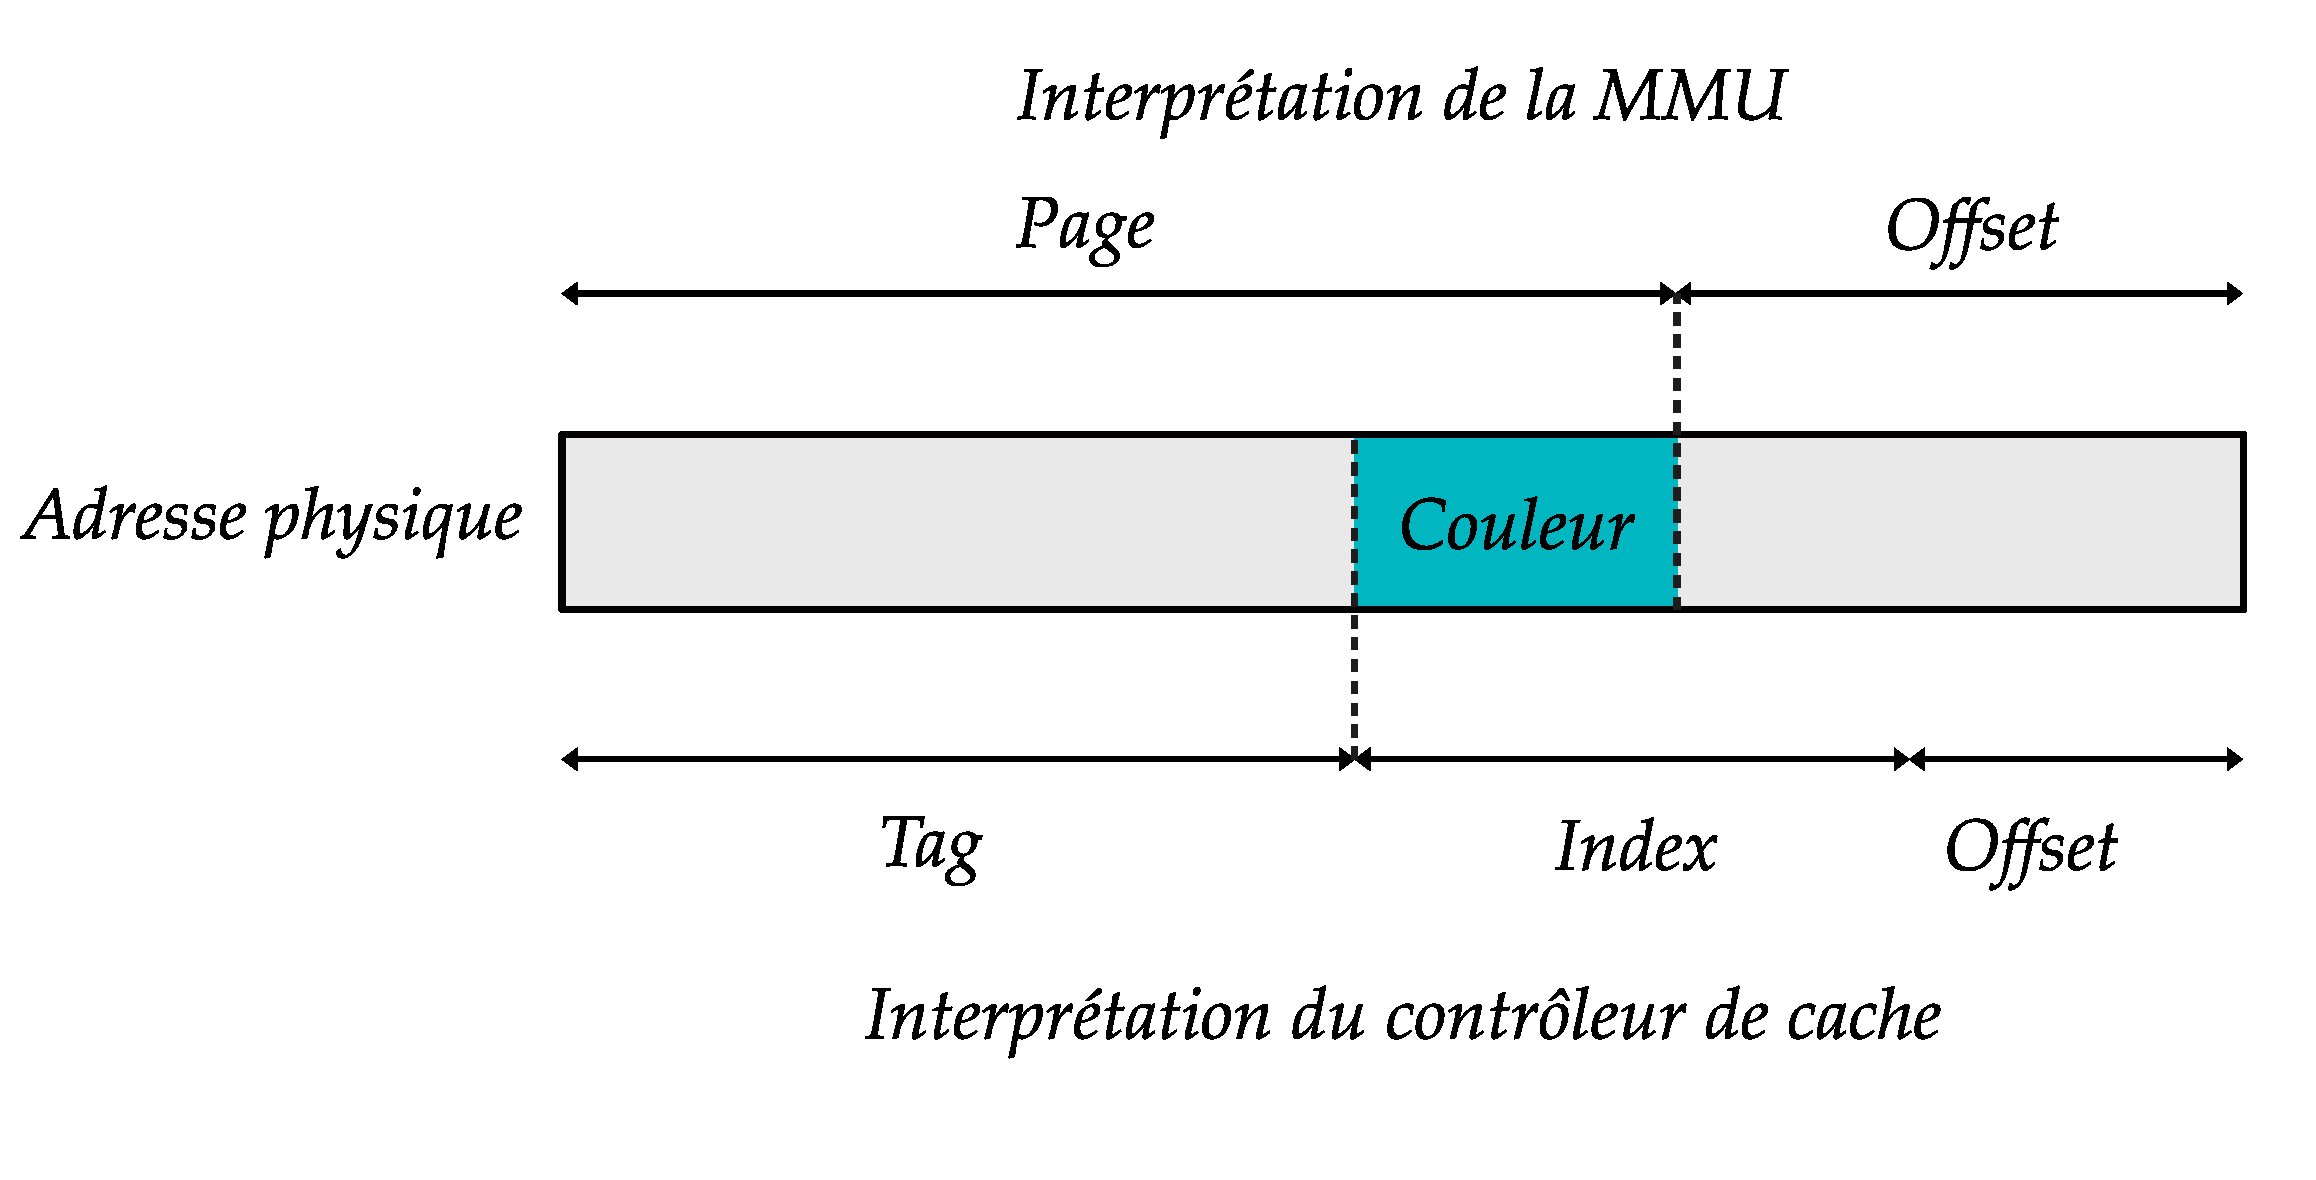
\includegraphics[width=0.65\linewidth]{graphics/figures/coloring.pdf}
	\caption{\label{fig:coloring}Bits de couleurs utilisés pour la coloration de cache}
\end{figure}

%Coloration de page. Technique logiciel. Association page virtuelle page physique. Encodage couleur dans addresse physiques. bits de pages. Utilisé en mono-coeur pour optimiser les caches. En multi-coeur permet de partitionner le cache en attribuant des couleurs disjointes entre les différents coeurs. Extension à d'autres types de ressources.

En pratique, l'application de la coloration de page se heurte à plusieurs difficultés.
Tout d'abord, pour utiliser cette technique il faut savoir comment les adresses sont interprétées par les différents composants que l'on souhaite partitionner.
Cette information n'est pas toujours disponible.
Des approches de rétro-ingénierie~\cite{yun2014palloc,panchamukhi_providing_2015} ont néanmoins été proposées pour pallier ce manque d'information.
Elles se basent sur l'étude du temps de réponse d'accès mémoire en fonction des adresses accédées.
L'arrivée des fonctions de hachages pour indexer les caches pose de nouveaux problèmes à la mise en œuvre de la coloration de cache.
Ces fonctions transparentes pour l'utilisateur ont une influence non négligeable sur les performances.
Ainsi, elles constituent souvent un secret industriel et doivent être identifiées par rétro-ingénierie~\cite{yarom2015mapping}.
De plus, même en connaissant la fonction de hachage, il n'est à connaissance pas possible de colorer des caches indexés de la sorte.

La coloration de pages est un mécanisme nécessitant du support au niveau de l'allocateur de pages physiques du système d'exploitation.
Or, ce mécanisme a des inconvénients pouvant dissuader les développeurs de systèmes d'exploitation d'implanter le support nécessaire à sa mise en œuvre.
C'est par exemple le cas dans le noyau \textsc{Linux}~\cite{torvald2003coloring}.
Les raisons invoquées sont une allocation de pages physiques rendue plus complexe et de possibles augmentations de la pression mémoire~\footnote{Zhang et al. ont montré que ce dernier point pouvait être évité en n'employant la coloration que sur les pages les plus utilisées~\cite{zhang2009towards}. Bien que prometteuse, cette solution rend d'autant plus complexe l'allocation de page physique.}.
Pour employer la coloration de pages sur ces systèmes, il faut donc utiliser un allocateur de pages spécifique.
À cette fin, Yun et al. ont proposé \textsc{PALLOC}~\cite{yun2014palloc}, un allocateur de page pour \textsc{Linux} gérant la coloration de pages.


% Elle rends l'allocation de pages physiques plus complexes, et peut augmenter la pression mémoire (bien que Zhang et al. ont montré que ce problème pouvait être contourné en utilisant la coloration que sur les pages les plus utilisées~\cite{zhang2009towards}).
% Pour ces raisons, elle n'est pas implantées dans tout les systèmes d'exploitation, notamment Linux~\cite{torvald2003coloring}.
% Pour supporter la coloration de page sous Linux, il faut donc passer par un allocateur de page spécifique comme PALLOC~\cite{yun2014palloc}.

%Nécessite de connaitre le mapping. Pas toujours possible. Notamment avec fonction de hachage pour indexation. Support OS pour coloration pas toujours disponible. Complexifie allocation de page physique. Augmentation de la pression mémoire. PALLOC réponse aux deux problèmes. Allocateur de page pour linux. Détection des mappings addresse matériel.
\paragraph{Support matériel}

Certaines architectures offrent du support matériel pour l'isolation spatiale, notamment dans les caches avec les fonctionnalités de verrouillage de lignes et de verrouillage de voies.
Le verrouillage de lignes permet de protéger spécifiquement une donnée.
Tandis que le verrouillage par voie permet d'empêcher la sélection de certaines voies par l'algorithme de remplacement.
Cette dernière méthode est généralement préférée, dans la mesure où elle ne nécessite pas de spécifier quelles données sont verrouillées.
Le verrouillage de voies peut être utilisé conjointement à la coloration de page afin de permettre un partitionnement à la granularité d'une page~\cite{mancuso2013real}.

\subsubsection{Conclusions}

Dans les systèmes temps-réel, le gain de déterminisme apporté par l'isolation spatiale a des avantages, en permettant par exemple de simplifier certaines analyses, mais aussi des inconvénients. 
L'isolation spatiale apporte un gain de déterminisme qui peut être coûteux en termes de performance en isolation.
Ce compromis a été étudié par Kim et al.~\cite{kim2017attacking} et Blin et al.~\cite{blin2016maximizing}, qui ont tous les deux conclu à de meilleures performances avec l'isolation spatiale.
Un autre problème est la gestion des couleurs au sein du système.
À cet effet, Ward et al. propose de considérer les couleurs comme des ressources partagées.
Et propose une analyse d'ordonnancement associée, se basant sur le principe d'équivalence avec un système mono-cœur~\cite{ward2013outstanding}.


%Support matériel. Verrouillage par ligne et par voies. Par ligne, verrouillage explicite des données. Par voie, plus utilisé. Permet de désigner les voies utilisés dans la politique de remplacement du cache. Utilisation conjointe avec la coloration de page permet une bonne granularité.

% Partitionement en temps réel. Gain de déterminisme vs perte de performance. Support des couleurs WARD. limité au cache. ANalyse d'ordonancement en considérant couleurs comme ressource partagée.
% Analyses font des hypothèse. En particulier sur la DRAM.

\subsubsection{Isolation temporelle}

L'isolation temporelle a pour but d'empêcher l'accès simultané à une ressource, en allouant des fenêtres de temps à chaque cœur (polititque TDMA~\footnote{Time Division Multiple Access}).
Nous ne parlerons ici que des méthodes logicielles, que l'on peut qualifier de méthodes de contrôle~\cite{girbal2015deterministic}.

% Approche de controle selon Girbal et al. Mise en oeuvre de politique TDMA en logiciel. Plus dur à mettre en oeuvre efficacement qu'isolation spatiale.

Une première approche de contrôle est l'approche tout ou rien, illustrée dans la figure~\ref{fig:tout_ou_rien}.
Celle-ci s'applique dans les systèmes à criticité mixte~\cite{vestal2007preemptive}, dans lesquels des tâches non critiques peuvent être soumises à des interférences (les tâches $PR1, PR3, PR4$ de la figure~\ref{fig:tout_ou_rien}) et des tâches critiques doivent absolument être isolées (la tâche $PR2$).
Cette approche peut être décrite par la règle suivante:
\begin{enumerate}
	\item Si une tâche critique est ordonnancée sur un cœur, les tâches de tous les autres cœurs doivent être suspendues.
	\item Lorsque des tâches non critiques s'exécutent, les tâches critiques sont suspendues.
\end{enumerate}
Ainsi, on peut s'assurer que les tâches critiques ne souffrent pas d'interférences.
Cette approche a notamment été utilisée dans l'hyperviseur temps-réel \textsc{PikeOS} \textsc~\cite{pikeOS} pour obtenir , sur un processeur bi-cœur, le plus haut niveau de certification dans un contexte ferroviaire~\cite{fisher2013certifying}.
%Bien qu'offrant une isolation parfaite à l'application temps-réel, cette approche est aussi très inefficace car elle ne permet d'exploiter qu'un seul coeur à la fois pour l'exécution  d'applications critiques.

% Par l'ordonancement. Criticité mixte. Application non critique peuvent subir des interférences. Pas les applications critiques. Application critique exécutée en isolation => applications non critique suspendues. Utilisé par PikeOS. A permis certification dans le ferroviaire pour un bi-coeur. Inneficace.

\begin{figure}
	\centering
	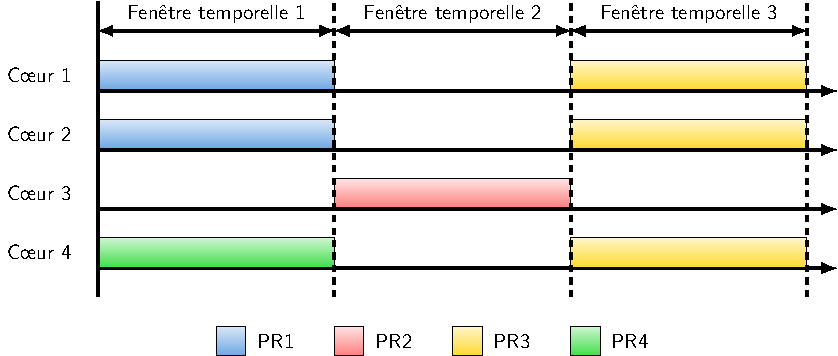
\includegraphics[width=\linewidth]{graphics/figures/tout_rien.pdf}
	\caption{\label{fig:tout_ou_rien}Ordonnancement tout ou rien}
\end{figure}

Si elle offre une isolation parfaite aux applications critiques, la solution employée dans \textsc{PikeOS} ne permet pas aux applications critiques de bénéficier du parallélisme.
Une meilleure utilisation des ressources est possible en faisant des hypothèses sur l'exécution des tâches.
Des modèles d'exécution, comme le superblock~\cite{durrieu2014predictable,schranzhofer2011timing}, ou PREM~\cite{pellizzoni2011predictable} permettent de diviser les applications en phases de communication et en phases d'exécutions.
Durant les phases de communications, l'application peut utiliser des ressources partagées.
Tandis que dans les phases d'exécution, l'application n'utilise que des ressources locales à un cœur.
Un ordonnancement des différentes phases est ensuite effectué, en permettant l'exécution en parallèle des phases d'exécutions et en s'assurant de l'exécution séquentielle des phases de communications (figure~\ref{fig:prem}).
Ce type de modèle a été utilisé dans de multiples travaux sur l'ordonnancement dit \emph{memory centric}~\cite{yao2012memory,2012_bak_memory,2014_alhammad_schedulability}.
Rivas et al.~\cite{rivas2019implementation} détaillent l'implantation du support pour le modèle PREM, dans le système d'exploitation temps-réel multi-cœur Hiperros~\cite{hipperos}~\cite{rivas2019implementation}.
Ce type de modèle permet d'améliorer la granularité de l'isolation temporelle, en permettant le parallélisme sur les phases d'exécutions.
Il nécessite par contre des adaptations du logiciel, rendant ce type d'approche incompatible avec des logiciels patrimoniaux.

%Modèle d'exécution. Superblock, ou PREM. Division de l'application en phases. Distinction entre phases d'exécution et de communications.Phase d'exécution utilise des ressources locales. Phases de communication utilise la mémoire.Ordonancement des phases d'exécution en parallèle. Ordonancement séquentiel des phases de communication. Plus efficace que l'approche tout ou rien. Pas compatible toutes les applications. Granularité de l'ordonancement. Sous utilisaiton du matériel malgré tout.

\begin{figure}
	\centering
	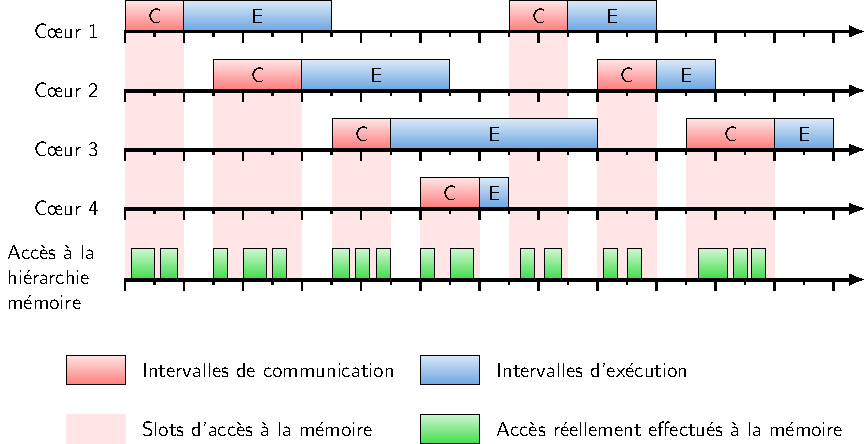
\includegraphics[width=\linewidth]{graphics/figures/prem.pdf}
	\caption{\label{fig:prem}Ordonnancement d'une tâche avec un modèle d'exécution déterministe}
\end{figure}

\textsc{MARTHy}~\cite{jean2015hypervisor} est un logiciel de contrôle permettant de mettre en œuvre une politique d'accès TDMA vers la mémoire dans un hyperviseur.
Le contrôle des accès est réalisé à l'aide d'une stratégie de programmation de la MMU et de fonctionnalités de verrouillage de cache.
L'idée est de maintenir l'invariant que toute page disposant d'une traduction valide est présente et verrouillée dans le cache.
Lorsqu'une application tente d'accéder à une donnée qui n'est pas présente en cache, une interruption de défaut de page est levée:
\begin{enumerate}
	\item Une exception de défaut de page est levée, donnant ainsi la main à l'hyperviseur (Marthy).
	\item Un emplacement pour accueillir la page à charger est sélectionné. 
	Dans la majeure partie des cas, cette étape consiste à sélectionner une page à évincer.
	\item L'hyperviseur attend le début d'une fenêtre temporelle durant laquelle il est autorisé à accéder à la mémoire.
	\item La page est chargée durant la fenêtre.
\end{enumerate}

\textsc{MARTHy} permet donc de bénéficier des avantages apportés par les modèles d'exécutions déterministes sur tout type d'application.
Cette approche néanmoins dégrade significativement les performances lorsque le mécanisme de contrôle est très sollicité.
De plus, sa mise en œuvre nécessite des fonctionnalités de verrouillage de cache, qui ne sont pas toujours disponibles.

%Système de controle permettant d'implanter une politique TDMA.
%Maintenance de l'invariant: toute page avec une correspondance valide est présente et verrouillée en cache. Sur défaut de page attente d'une fenetre temporelle. Implantée dans PowerPC. Repose sur la possibilité de gérer TLB en soft. problème de performances.

\begin{figure}
	\centering
	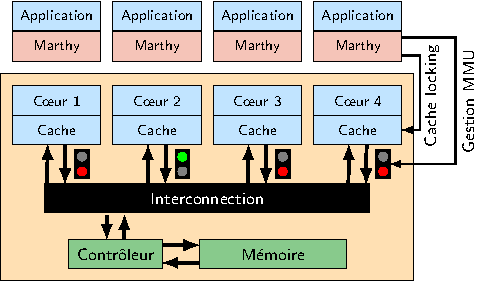
\includegraphics[width=0.75\linewidth]{graphics/figures/marthy.pdf}
	\caption{\label{fig:marthy}\textsc{MARTHy}}
\end{figure}

\subsubsection{Conclusions}

L'isolation temporelle a l'avantage d'offrir beaucoup de déterminisme en éliminant les accès simultanés aux ressources partagées.
Ce déterminisme est néanmoins acquis au prix d'une sous utilisation du matériel.
Elle s'avère néanmoins difficile à mettre en œuvre.
Les modèles d'exécutions déterministes sont une piste prometteuse pour les applications futures.
Néanmoins, il n'est pas certain que toutes les applications puissent être écrites pour satisfaire à ce genre de modèle.
Une question demeure sur la granularité du contrôle des accès.
Si une granularité plus fine peut permettre une meilleure utilisation du matériel, le coût du contrôle augmente également.
À notre connaissance, il n'y a pour le moment pas de réponse claire au problème du coût de contrôle dans la littérature.
% Isolation temporelle => Déterministe. Sous utilisation du matériel. Difficulté de mise en oeuvre.

\subsection{Systèmes de régulation}

L'isolation des différents cœurs, qu’elle soit spatiale ou temporelle, offre du déterminisme au prix d'une dégradation des performances.
Selon le niveau de charge du système, le gain de déterminisme peut ne pas justifier ce coût.
Le but des \emph{systèmes de régulation} est d'adapter le niveau d'isolation pour les tâches temps-réel en fonction de la pression effectivement exercée sur les ressources partagées.
Nous distinguons deux composants majeurs dans ces systèmes:
\begin{itemize}
	\item Un \emph{plan de données}, en charge de déterminer s’ il y a un risque de dépassement d'échéance en fonction de l'état observé du système.
	\item Un \emph{plan de contrôle}, en charge de rétablir un domaine de fonctionnement sûr en cas d'alerte du plan de données.
\end{itemize}
Ce type de solutions est plutôt adapté à des systèmes à criticité mixte, car dans ce type de systèmes des tâches non critiques peuvent être suspendues pour permettre aux taches critiques de respecter leurs échéances.

%Régulation : limiter l'impact des interférences. Deux composants: plan de données => monitorage du retards. Plan de contrôle => rétablissement d'une situation sûre. Mode dégradé. Type d'approche plutot adaptée aux systèmes à criticité mixte.

Une première approche consiste à réguler l'accès aux ressources.
C'est ce que permettent les \emph{régulateurs de bandes passantes}, tels que MRS~\cite{inam2014multi} ou MemGuard~\cite{yun2013memguard}.
Ces régulateurs fonctionnent sur le principe d'un \emph{serveur périodique}.
Chaque cœur se voit attribuer un budget d'accès autorisés sur une \emph{période de régulation}.
Les éventuels dépassements de budgets sont détectés à l'aide de \emph{compteurs de performances}.
Des compteurs de performances sont utilisés pour détecter le dépassement de budget éventuel.
En pratique, ces compteurs sont programmés pour lever une interruption lorsqu'ils sont saturés et initialisés à leur valeur maximale moins le budget alloué.
Lors d'un dépassement de budget, le cœur concerné est mis en attente jusqu'à la période de régulation suivante.

Ce type d'approche peut être utilisée pour simplifier l'analyse d'ordonnancement d'un système~\cite{pellizzoni2016memory,agrawal2017contention}.
La mise en œuvre d'un régulateur de bande passante dépend directement des événements observables sur le matériel utilisé.
Notons que cette observation doit se faire indépendamment pour chaque cœur.
Ce n'est pas toujours possible sur les cibles COTS.
En effet, dans ces dernières, les ressources partagées ne sont généralement observables qu'au moyen d'un compteur global ne permettant pas de différencier la consommation des différents cœurs.

De plus, le bon fonctionnement de ce type d'approche dépend directement du dimensionnement du système et donc des budgets alloués aux différents cœurs.
En particulier, il n'y a pas de notion de sensibilité.
C'est-à-dire que si le dimensionnement du système est trop optimiste, rien ne garantit le respect des échéances temporelles.
MemGuard apporte une solution à ce problème en définissant un seuil maximal d'utilisation du bus mémoire permettant de garantir le respect des échéances, ce qui pose un problème de sous utilisation des ressources.

%La régulation en tant que telle nécessite donc de sous-utiliser les ressources pour être sure.

%Régulation de bande passante. Permet de limiter l'aggressivité des applications. MemGuard et MRS.Principe d'un serveur périodique. Chaque coeur a un budget de consommation: nombre d'accès max par période. Budget renouvelée au début de chaque periode de régulation. Consommation mémoire mesurée avec compteur de performances. Exceptions levée sur overflow. Quand exception suspension des taches sur le coeur jusqu'à la prochaine période de régulation. Nécessite d'avoir les évenements pertinents. Pas de notion de sensibilité. Plus d'interférences -> Moins de consommation.MemGuard utilise un seuil global. Sous utilisation. Utilisé par certaine études WCET.

\begin{figure}
	\centering
	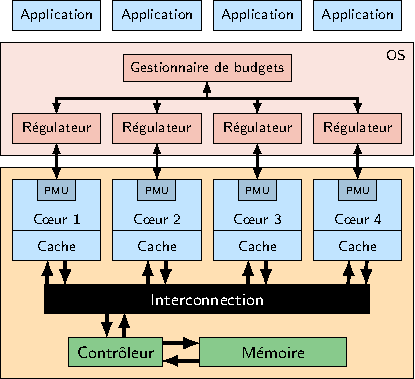
\includegraphics[width=0.6\linewidth]{graphics/figures/memguard.pdf}
	\caption{\label{fig:memguard}MemGuard}
\end{figure}

Le \emph{Contrôleur de WCET distribué}~\cite{kritikakou2014run,kritikakou2014distributed} est une approche de régulation dont le plan de contrôle n'est pas focalisé sur l'utilisation des ressources, mais sur le retard pris par les tâches temps-réel.
Cette approche concerne les systèmes à criticité mixte.
Des \emph{points de contrôles} sont injectés dans les applications temps-réel du système.
Ces points de contrôle comprennent une \emph{condition de sûreté} permettant de vérifier que la tâche peut respecter ses échéances malgré la contention.
Si la condition de sûreté d'un point de contrôle n'est pas respectée, alors une notification est envoyée à un \emph{contrôleur de WCET} qui en réponse va suspendre les tâches non critiques du système.
La principale difficulté dans la mise en œuvre de ce type d'approche est le placement des points de contrôles et la spécification des conditions de sûreté.
% Lorsqu'ils sont exécutés, ces points de contrôle vériefie une \emph{condition de sureté} et notifie un \emph{contrôleur de WCET} si celle 

%Distributed WCET controler. Solutions pour système à criticité mixte. Injection de points de contrôles dans le code des applications. Point de contrôles s'assure du respect des échéances temporelles. Si condition de sureté non remplie, tâches non critiques suspendues. Pb placements des points et validité des conditions de sureté. 

\begin{figure}
	\centering
	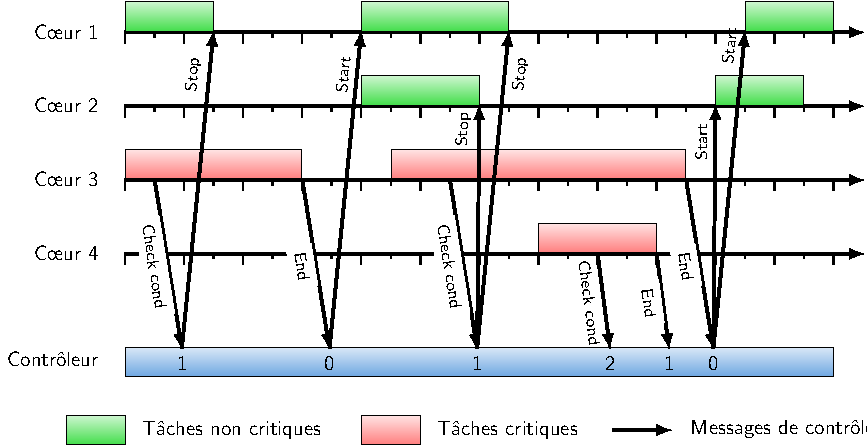
\includegraphics[width=\linewidth]{graphics/figures/kri.pdf}
	\caption{\label{fig:kritikakou}Contrôleur de WCET distribué}
\end{figure}

La solution proposée par Blin et al.~\cite{blin2016maximizing} vise à maintenir le retard subi par une application en dessous d'un seuil déterminé lors de la conception du système.
Tout comme le contrôleur de WCET distribué, cette approche s'applique à des systèmes à criticité mixte et suspend les tâches non critiques lorsque le seuil de retard spécifié est atteint.
Ce mécanisme n'exige pas compteurs locaux, mais un compteur global, la rendant compatible avec la plupart des cibles COTS.
Elle est néanmoins limitée au cas où seul un cœur exécute des applications temps-réels.
Ce système repose sur trois grandes étapes. Deux étapes hors-ligne permettent de définir le plan de données, tandis que la troisième étape en ligne implante le plan de contrôle:
\begin{enumerate}
	\item \emph{Modèle de retards de la plateforme matérielle}. Cette étape consiste à définir une fonction, permettant d'associer un surcoût temporel à une consommation de bande passante en isolation et une bande passante globale observée.
	Cette fonction est conservative et construite à partir de données expérimentales.
	De multiples expériences sont effectuées avec des microbenchmarks, et seuls les cas les plus pessimistes sont retenus.
	\item \emph{Modèle de consommation de l'application à protéger}. Dans cette étape, la consommation de bande passante d'une application est mesurée en isolation.
	Les mesures sont effectuées sur différentes phases de l'application.
	\item \emph{Contrôle en ligne} À l'exécution, un mécanisme de contrôle mesure la bande globale et détermine le retard subi par l'application temps-réel en utilisant les deux modèles constituant le plan de données.
	Lorsque le retard cumulé est trop élevé, les applications non temps-réels sont suspendues.
\end{enumerate}

La mise en œuvre efficace de ce type d'approche dépend grandement de la qualité du plan de données que l'on a pu définir.
Plus le modèle de retards est imprécis, plus vite les applications non critiques sont suspendues, ce qui résulte dans une utilisation moindre du matériel.
Une meilleure précision du modèle de retards peut donc conduire à une meilleure utilisation du matériel.

\subsubsection{Conclusions}

Les systèmes de régulation permettent d'adapter le niveau d'isolation du système en fonction de l'utilisation globale des ressources matérielles.
Ces approches offrent donc un compromis entre déterminisme et efficacité, ce qui les rend particulièrement attractives pour des applications industrielles.
L'implantation efficace de tel système demeure néanmoins un défi important.
Un verrou technologique important réside notamment dans le plan de données en charge de détecter les situations à risque.
En effet, pouvoir détecter précisément ces situations détermine directement la confiance que l'on peut avoir dans ces approches et éviter les surdimensionnements excessifs.

% Régulation permet de fournir un filet de sécurité. Plutot adapté à des système à criticité mixte où on peut mettre en place un mode dégradé.
% Plan de donnée critique. Permet de détecter précisemment situations à risque. Dimmensionnement du système important.
\section{Conclusions du chapitre}

Nous avons dans ce chapitre présenté l'impact des interférences dans le cadre des systèmes temps-réels.
Prendre en compte les interférences lors de la conception des systèmes temps-réels revient à surdimensionner ces derniers.
En effet, le dimensionnement de ces systèmes doit correspondre aux pires cas.
La complexité et l'opacité du matériel moderne rendent ces interférences difficilement prévisibles et conduisent à des surdimensionnements inacceptablement pessimistes des systèmes.

À l'heure actuelle, les approches traditionnellement employées pour l'analyse de pire temps d'exécutions sont mises en échec par le problème des interférences.
Il est possible dans certains cas d'améliorer l'isolation des différents, mais cela se fait au détriment des performances.
Enfin, des approches de régulation permettent d'obtenir un compromis intéressant entre déterminisme et performances, mais leur mise en œuvre nécessite d'anticiper efficacement le retard subi à cause des interférences.

Dans le reste de ce document, nous présentons nos travaux dont le but est de caractériser la sensibilité aux interférences des applications à partir d'une caractérisation de leur comportement exécutée seules.
Le but est de pouvoir estimer à priori le retard que peut subir un programme, mais aussi de permettre, à terme, la conception de 
systèmes de régulation efficaces.
% Autre approche proposée par Blin et al. Meme principe que Kritikakou. Condition de sureté basés sur la consommmation. 3 étape deux hors ligne, 1 en ligne. Caractérisation de la consommation mémoire. Modèle de retards. 